\section{Conference Venue}

 \begin{figure}[h!]
  \centering
      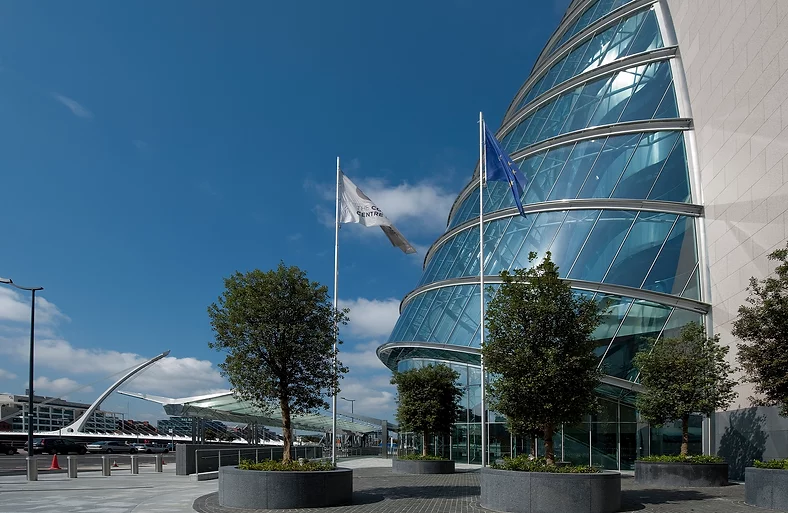
\includegraphics[width=0.9\linewidth]{/Users/uniba/Documents/GitHub/aclpub2/examples/handbook_acl/local_guide/images/location.png}
 \end{figure}

Venue.
\section{About Ireland}

About.
\section{About Dublin}

 \begin{figure}[h!]
  \centering
      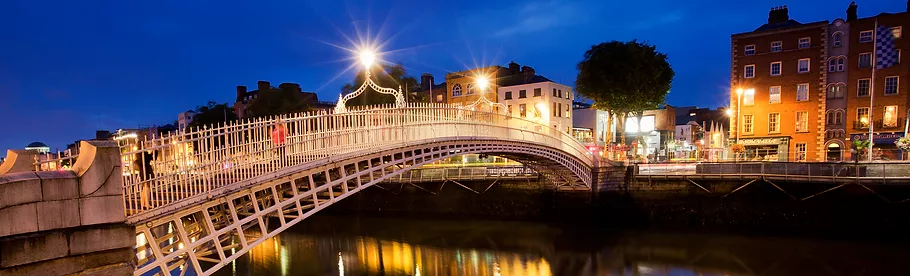
\includegraphics[width=0.9\linewidth]{/Users/uniba/Documents/GitHub/aclpub2/examples/handbook_acl/local_guide/images/dublin.png}
 \end{figure}
 \leavevmode\newline

Info. \\

\section{Enjoying Ireland}

 \begin{figure}[h!]
  \centering
      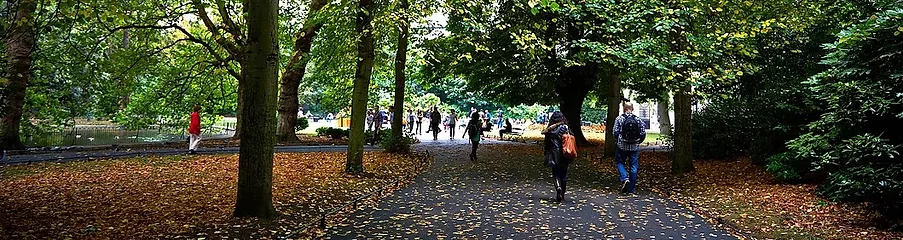
\includegraphics[width=0.9\linewidth]{/Users/uniba/Documents/GitHub/aclpub2/examples/handbook_acl/local_guide/images/green.png}
 \end{figure}
 \leavevmode\newline

{\Large \textit{Top Visitor Attractions}}\\
Attractions. \\


 \leavevmode\newline
\section{Useful Information}

{\large \textbf{Electricity}}\\
220 / 240 volts . 3 Pin Plug.\\

{\large \textbf{Driving in Ireland}}\\
Traffic in Ireland drives on the left.\\

{\large \textbf{Insurance}}\\
The Conference Organising Committee or its agents will not be responsible for any medical expenses, loss or accidents incurred during the conference. Delegates are strongly advised to arrange their own personal insurance to cover medical and other expenses including accident or loss. Where a delegate has to cancel for medical reasons, the normal cancellation policy will apply. It is recommended that citizens from EU countries bring with them a current European Health Insurance Card (EHIC) card.\\

{\large \textbf{Language}}\\
The main languages are English and Irish and most signposts in the Republic are bilingual. English is spoken by everyone while Irish is generally confined to pockets of the south-west, west and north-western coastal areas.\\

{\large \textbf{Money}}\\
The Euro is the currency in the Republic of Ireland. The Euro has 100 cents in the euro with coins in denominations of 1, 2, 5, 10, 20 \& 50 cents and 1 and 2 euros. Euro notes come in denominations of 5, 10, 20, 50, 100, 200 and 500 euro. Foreign exchange bureaus are available in most banks, post offices, Tourist Information Offices, airports, some shops and accommodation. Bureau de Change kiosks are also situated in many towns and most cities. There are no exchange controls in Ireland. Any sums of money in any currency can be freely brought into or taken out of the country without disclosure or other formalities.\\

{\large \textbf{Smoking}}\\
Under current legislation, smoking is banned in all public areas and work places, including restaurants, pubs and bars. Smoking is still permitted in hotel bedrooms which are designated as smoking bedrooms by the hotel. Smoking in bedrooms in guest houses and bed and breakfast accommodation is at the discretion of the owner. There are substantial penalties in place for those found to be in breach of these regulations.\\

{\large \textbf{Tax}}\\
Refunds Value Added Tax (VAT) is charged at 23\% on most goods. Cash back is the simplest and most widely used VAT refund service that issues cash refunds on departure for a handling fee. Ask for cash back form when you make your purchase.\\

{\large \textbf{Time}\\
\normalsize
From November until February, Ireland operates on GMT 0 hour Greenwich Mean Time. From March to October, Ireland operates on GMT Greenwich Mean Time + 1 hour.\\

{\large \textbf{Shopping}}\\
Dublin has a busy city centre shopping area around Grafton Street and Henry Street. There is a huge range of products to bring home – from traditional Irish hand-made crafts to international designer labels. Shopping hours in general are from 9.00am to 6.00pm Monday to Saturday, with shops open until 8.00pm on Thursdays, and many shops open from 2.00pm – 6.00pm on Sunday. Dundrum Town Centre is a large shopping centre located in South Dublin. The LUAS Green Line serves Dundrum Town Centre from St. Stephens Green to Brides Glen. The Dundrum and Balally stops are only a few minutes-walk from the centre.\\

{\large \textbf{Tipping}}\\
Hotels and restaurants often add 10-15\% to the bill especially for large parties. This is not mandatory in the Republic of Ireland. Tip cabs 10\% and porters 60c per bag.\\

{\large \textbf{Weather}}\\
Ireland enjoys a temperate climate, with mild winters and relatively cool summers. The daily temperature in May in Dublin is on average 15 degrees Celsius.
Dublin enjoys reasonable sunshine and rain belts reaching the east coast are frequently light and generally clear within a few hours. It is always wise when travelling to Ireland to pack rain gear or an umbrella.\\

\section{Visa \& Passport}
Visa.

{\large \textbf{Do I need a visa?}}\\
Please consult with the relevant Irish Embassy/Consulate/Visa Office or visit the official government website: \\
\url{https://www.dfa.ie/travel/visas/visas-for-ireland/}

 \leavevmode\newline
\section{Covid-19 Safety}
Covid.

{\large \textbf{Measures in place}}
\begin{itemize}
 \item A specific Covid-19 policy in place.
\end{itemize}

{\large \textbf{Staying safe}}\\
Rules.

 \leavevmode\newline
\section{Travel to the Conference Venue}

 \begin{figure}[h!]
  \centering
      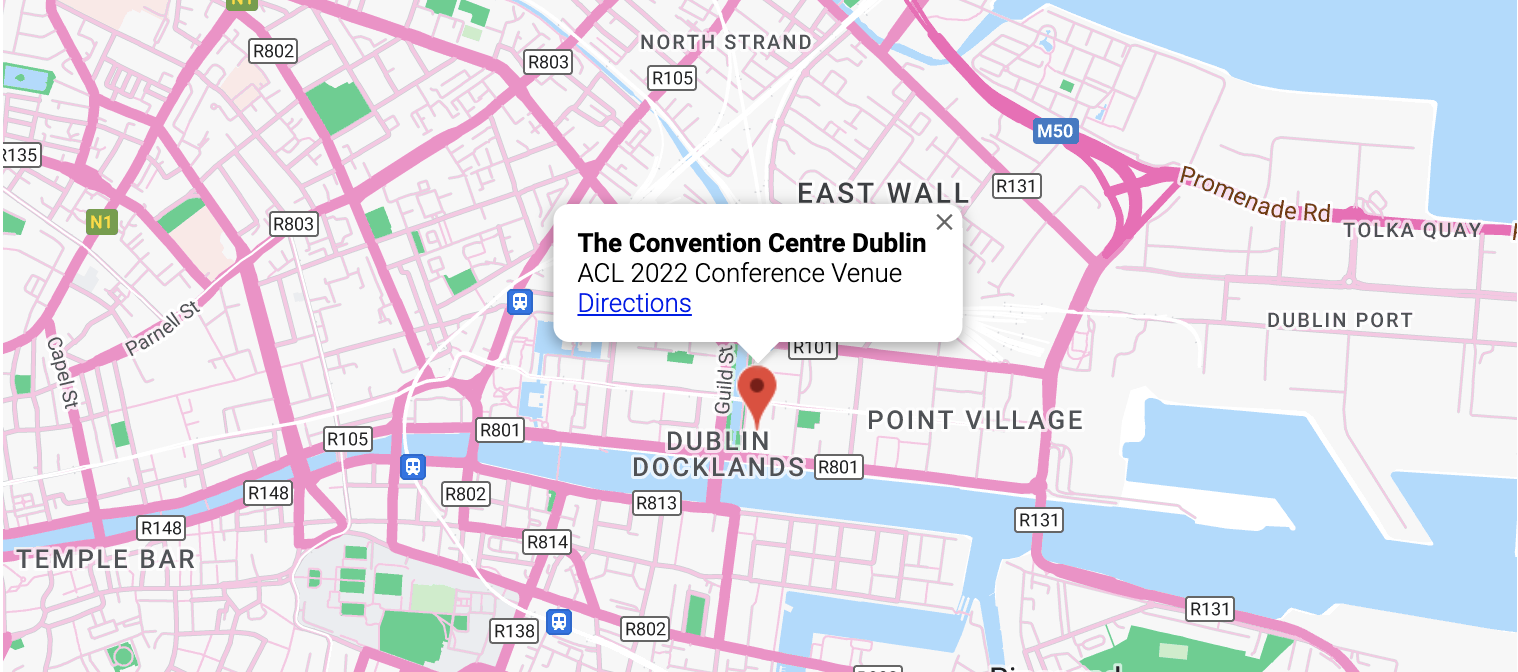
\includegraphics[width=0.9\linewidth]{/Users/uniba/Documents/GitHub/aclpub2/examples/handbook_acl2022/local_guide/images/map.png}
 \end{figure}
 \leavevmode\newline
Travel.